\xchapter{Avaliação da disponibilidade de código-fonte dos softwares científicos}
{Este capítulo apresenta a caracterização dos softwares científicos de análise
estática de código-fonte quanto à sua disponibilidade de código-fonte.}
\label{caracterizacao-ferramentas}

% Introduction
% Background
% Experimental Setup (hipoteses / design)
% Results (data analysis)
% Discussion
% Threats to validity
% Conclusions

Muitos estudos em engenharia de software sofrem de dificuldades de repetição
\cite{Tang2016}, uma prática importante para aumentar a validade científica dos
estudos e seus resultados. {\it Repetição} é a atividade de refazer exatamente
o que outra pessoa fez usando os artefatos originais, a disponibilidade de
código-fonte é o requisito mínimo para possibilitar tal prática.

Avaliar e caracterizar a disponibilidade dos {\it softwares cientificos}
publicados em conferências de engenharia de software, com especial atenção à
disponibilidade do seu código-fonte, é útil para evidenciar o quão possível é
repetir tais estudos e assim aumentar a validade em seus resultados.

Desta forma, este estudo tem como objetivo geral avaliar a disponibilidade dos
softwares científicos publicados em conferências de engenharia de software e
assim evidenciar o quanto tais estudos sofrem com dificuldades de repetição.

Esta avaliação e caracterização será focada em publicações da área de análise
estática de código-fonte visto que seria inviável no escopo deste trabalho
englobar todas as áreas de pesquisa da engenharia de software.

A área de análise estática de código-fonte possui carência de estudos avaliando
suas ferramentas, desta forma conseguiremos contribuir com esta área ao mesmo
tempo que exploramos o quanto os pesquisadores publicando softwares nesta área
publicam e disponibilizam seus softwares contribuindo para a divulgação dos
resultados e proporcionam repetição dos seus estudos.

\section{Planejamento do estudo}

\subsection{Seleção de softwares científicos}

A seleção de {\it softwares científicos} será realizado através de uma {\it
revisão estruturada}, um processo disciplinado para busca e seleção de
softwares de um domínio específico publicados em artigos acadêmicos a partir de
critérios bem definidos, de forma que seja possível a reprodução do estudo por
parte de pesquisadores interessados.

A revisão estruturada difere da revisão e do mapeamento sistemático por ser um
processo mais simples e menos rígido, onde o resultado final é um conjunto de
softwares, enquanto no mapeamento ou na revisão sistemática há um esforço em
caracterizar os artigos analisados o mesmo não ocorre na revisão estruturada.

A revisão estruturada é organizada em três atividades de (1) busca de artigos
(definição das fontes, obtenção dos artigos nas fontes), (2) filtro (definição
de critérios de busca, definição de script de busca) e (3) seleção de artigos
com publicação de softwares. Estas atividades estão representadas na Figura
\ref{figura-revisao-estruturada}.

\begin{figure}[h]
  \center
  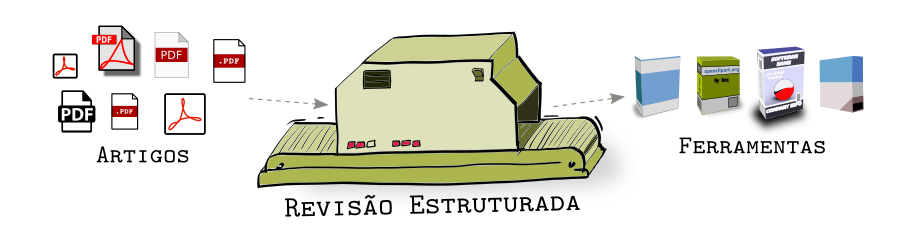
\includegraphics[scale=0.21]{imagens/revisao-estruturada.png}
  \caption{Atividades da revisão estruturada: (1) busca, (2) filtro e (3) seleção}
  \label{figura-revisao-estruturada}
\end{figure}

Na primeira atividade da revisão estruturada -- {\it (1) Busca} -- são definidas as fontes de entrada,
estas fontes são conferências que abordam o tema de interesse do estudo, e que
apresentam um grande potencial de encontrar softwares do domínio de aplicação
desejado, neste estudo o interesse está em softwares de análise estática de
código-fonte. Esta primeira atividade de busca deve incluir o maior número
possível de ediçoes das conferências selecionadas, para cada edição são
copiados localmente todos os artigos em formato PDF para posterior filtro na
atividade subsequente.

A segunda atividade da revisão estruturada -- {\it (2) Filtro} -- realizada em cima de todo o conjunto
de artigos é um filtro automático que busca em todo o conteúdo dos artigos os
termos de interesse, estes termos devem ser pensados em relaçao ao domínio de
aplicação desejado, devem ser abrangentes a fim de evitar falsos negativos.
Os seguintes termos serão utilizados neste filtro:

\begin{verbatim}
  "tool" OU "framework"; E
  "download" OU "available"; E
  "http" OU "ftp"; E
  "static analysis" OU "parser".
\end{verbatim}

Estes termos devem encontrar artigos com publicação de {\it softwares
científicos} do domínio de análise estática de código-fonte com disponibilidade
para {\it download}, seja binário ou código-fonte.

A terceira e última atividade da revisão estruturada -- {\it (3) Seleção} --
identifica se cada artigo resulta, de fato, em publicação de {\it
software científico} do domínio de aplicação desejado. Esta seleção é feita a
partir de uma leitura superficial do artigo em busca de indícios de que o
artigo publica de fato algum software.

Nesta etapa cada artigo é lido, inicialmente apenas introdução, resultados e
conclusão com o objetivo de identificar se o artigo publica {\it software
científico} e indica onde obter uma cópia do software. {\it Softwares
científicos} que sejam mais abrangentes do que apenas análise estática de
código-fonte mas que contenham esta função em seu conjunto também são
selecionados.

\subsection{Avaliação da disponibilidade dos softwares científicos}

Os {\it softwares científicos} de análise estática de código-fonte selecionados
na revisão estruturada serão avaliados em relação à sua disponibilidade,
dois aspectos serão levados em conta nesta avaliação, um relacionado à como o
artigo apresenta e disponibiliza o {\it software científico} e
o outro relacionado a como o software está de fato disponível, ou seja, se a fonte
informada está funcional ou não.

O primeiro aspecto relacionado à como o artigo disponibiliza o software
científico será caracterizado como uma das seguintes opções:

\begin{itemize}
  \item Artigo não indica onde obter o software\\
    {\it \small artigo não indica fonte para obtenção do software}
  \item Fonte para obtenção do software indisponível\\
    {\it \small artigo indica fonte mas encontra-se inacessível, fora do ar ou com erros}
  \item Software disponivel, binários ou código-fonte\\
    {\it \small a fonte indicada está disponível e acessível}
\end{itemize}

Este primeiro aspecto tem a importância de mostrar quantos artigos falham em
não informar ao leitor qual ou quais são as fontes para obtenção dos artefatos
de software produzidos no estudo. A fonte indicada será acessada a fim de
identificar se está funcional e se é possível obter uma cópia do software.

%Mesmo que o autor tenha disponibilizado fontes para obtenção dos artefatos produzidos,
%o fato de não informarem a fonte inviabiliza, ou ao menos dificulta, bastante
%pesquisadores interessados em repetir ou reproduzir os resultados de tais estudos.

O segundo aspecto diz respeito à como o software está disponível e detalha o
primeiro aspecto informando de que forma os softwares estão disponíveis, podendo
ser:

\begin{itemize}
  \item Código Aberto ({\it Open Source})\\
    {\it \small a ferramenta é livre e o código-fonte está disponível}
  \item Grátis ({\it Free})\\
    {\it \small a ferramenta é grátis mas o código-fonte não está disponível}
  \item Comercial\\
    {\it \small a ferramenta está disponível mediante pagamento}
\end{itemize}

Vale lembrar que apenas os softwares caracterizados inicialmente como
{\it``Software disponivel, binários ou código-fonte''} serão detalhados aqui.
Este segundo aspecto toma como base o trabalho de \citeonline{Novak2010} em que
propõe uma taxonomia e um conjunto de dimensões para caracterização de
ferramentas de análise estática.

Os softwares caracterizados como ``Código Aberto ({\it Open Source})''
incluirão também softwares sem licença desde que tenham código-fonte
disponível, sabemos que isto contraria as definições de {\it livre} e
{\it open} da Free Software
Foundation\footnote{\url{https://www.gnu.org/philosophy/free-sw.html}} e Open
Source Initiative\footnote{\url{https://opensource.org/osd}}, respectivamente,
mas será feito assim pois o acesso ao código-fonte é a característica
de interesse neste estudo, com ele é possível estudar o
conhecimento empregado nos softwares, bem como repetir o estudo original
utilizando ou executando tal código quando necessário.

%Iremos
%utilizar a categoria relacionada à disponibilidade dos softwares que responde a
%pergunta: ``de que forma a ferramenta está disponível?''.
%
%Este aspecto está relacionado ao estado do software em relação à sua
%disponibilidade, e indica como o software está disponível, para os softwares
%com código-fonte disponível será avaliado e documentado qual licença o author
%utiliza.
%
%Vale lembrar que apenas os artigos que oferecem fonte para obtenção disponível,
%ou seja, endereços e links ainda funcionando, serão considerados na
%caracterização deste segundo aspecto.

A fonte de informação para a caracterização destes dois aspectos serão os
artigos relacionados aos softwares, o código-fonte, documentos e site do
projeto, quando disponíveis.

\section{Resultados}

Na {\it revisão estruturada} selecionamos a conferência SCAM - {\it
Source Code Analysis and Manipulation Working
Conference}\footnote{\url{http://www.ieee-scam.org}} e a conferência ASE - {\it
Automated Software Engineering}\footnote{\url{http://ase-conferences.org}},
ambas conferências com largo histórico de publicação sobre análise de
programas e apresentam um alto potencial de encontrar softwares do domínio de
análise estática de código-fonte.

A primeira atividade da revisão estruturada -- {\it (1) Busca} -- passa por
todas as ediçoes das duas conferências até o ano de 2015, uma lista completa
e o endereço de cada edição onde os artigos foram obtidos está documentado no
Apêndice \ref{edicoes-conferencias}, lá é indicado o endereço da conferência
nos respectivos portais onde os artigos foram obtidos. Todas as trilhas de
ambas as conferências foram incluídas, econtramos nesta atividade 1879 artigos, 346 artigos
do SCAM e 1533 artigos do ASE, 

A segunda atividade da revisão estruturada -- {\it (2) Filtro} -- realizada neste
conjunto de 1879 artigos em busca dos termos abaixo resultou em 436 artigos,
155 artigos da conferência SCAM e 281 da conferência ASE.

\begin{verbatim}
  "tool" OU "framework"; E
  "download" OU "available"; E
  "http" OU "ftp"; E
  "static analysis" OU "parser".
\end{verbatim}

A terceira e última atividade da revisão estruturada -- {\it (3) Seleção} --
realizada em cima dos 436 artigos selecionou 103 artigos com publicação de {\it software
científico} do domínio de aplicação de análise estática de código-fonte, 41 da
conferência SCAM e 62 da conferência ASE, as Tabelas \ref{artigos-do-scam} e
\ref{artigos-do-ase} detalham o total de cada conferência.

Assim, ao final da revisão estruturada encontramos um total de 103 artigos com
publicação de software de análise estática de código-fonte, estes 103 softwares
foram encontrados em meio aos 1879 artigos analisados,
uma lista com todos os 103 softwares e uma breve descrição de cada um é
apresentado na Tabela \ref{resumo-softwares}.

Estes 103 artigos publicam {\it softwares científicos} e na avaliação sobre
disponibilidade dos softwares foram caracterizados da seguinte forma:

\begin{table}[H]
\centering
\begin{tabular}{| l | l |}
  \hline
  {\bf Característica}                          & {\bf Número de artigos} \\
  \hline
  Artigo não indica onde obter o software       & 45 \\
  \hline
  Fonte para obtenção do software indisponível  & 23 \\
  \hline
  Software disponivel, binários ou código-fonte & 35 \\
  \hline
\end{tabular}
\end{table}

Estes 35 softwares caracterizados como {\it ``Software disponivel, binários ou
código-fonte''} foram avaliados em relação ao segundo aspecto em respeito à de
que forma os softwares estão disponíveis.

\begin{table}[H]
\centering
\begin{tabular}{| l | l |}
  \hline
  {\bf Característica}                          & {\bf Número de artigos} \\
  \hline
  ``Código Aberto ({\it Open Source})''         & 32 \\
  \hline
  ``Grátis ({\it Free})''                       & 3  \\
  \hline
  ``Comercial''                                 & 0  \\
  \hline
\end{tabular}
\end{table}

Ou seja, de um total de 103 artigos publicando softwares de análise estática de
código-fonte, apenas 32 artigos (31\%) estão disponíveis para download com
código-fonte, o que nos leva a conclusão que os 71 artigos (69\%) restantes não
podem ser repetidos considerando que disponibilizar o código-fonte dos
artefatos de software é o mínimo requisito para possibilitar tal prática.

\section{Ameaças à validade}

Estamos considerando que o código-fonte é necessário para repetir um dado
estudo mas pode ser que em alguns casos o estudo possa ser repetido mesmo sem a
disponibilidade do mesmo, isto poderia ser resolvido realizando a repetição
de cada estudo na prática e a partir daí identificar se o código-fonte dos
softwares desenvolvidos são requeridos.

A escolha de um domínio de aplicação específico para seleção dos softwares
pode ser um fator de influencia nos resultados obtidos, sendo possível que
o número de artigos com publicação de softwares com código-fonte disponível
encontrado não reflita nos outros domínios, os problemas diagnosticados
neste domínio pode não ser verdade em outros domínios, sendo necessário
realizar o mesmo estudo em outros domínios.

A leitura dos artigos na revisão estruturada para identificar se publicam
softwares de análise estática de código-fonte, se disponibilizam fonte para
obtenção de tais softwares, e se os softwares são mesmo do domínio de aplicação
de análise estática de código-fonte podem ter maior validade se feitos em
par e revisados por outros pesquisadores, neste estudo tudo foi feito pelo
autor deste estudo e não houve revisão por pesquisadores independentes.

\section{Conclusões}

Dos 346 artigos do SCAM e 1533 artigos do ASE analisados na revisão estruturada
apenas 44\% (155 artigos) e 18\% (281 artigos) continham os termos pesquisados
no filtro automático da segunda atividade da revisão, respectivamente.

Deste total apenas 11\% (41 artigos) e 4\% (62 artigos) foram selecionados na
terceira e última atividade da revisão contendo publicação de ferramenta de
análise estática.

Resultando em 103 artigos com publicação de {\it software científico} de
análise estática de código-fonte, apenas 35 possuem fonte para obtenção do
software, sendo 32 de código aberto, ou seja, com disponibilidade de
código-fonte, e 3 grátis, apenas binários disponível. Ou seja, apenas 31\% dos
artigos com publicação de software disponibilizam o código-fonte das mesmas.
Isto significa que 69\% dos artigos com publicação de software de análise
estática de código-fonte são potencialmente impossíveis de serem repetidos, já
que os artefatos originais são necessários para tal atividade e o artigo não
disponibiliza o código-fonte dos mesmos.

\subsection{Reproducibilidade do estudo}

Todas as atividades e artefatos produzidos neste estudo estão documentados em
repositório público no Github\footnote{GitHub é uma plataforma de hospedagem de
código para controle de versão e colaboração.} no seguinte endereço:

\begin{itemize}
  \item \url{http://github.com/joenio/dissertacao-ufba-2016}
\end{itemize}

Os artigos analisados na revisão estruturada estão todos documentados arquivo
{\it
dataset/dataset.ods}\footnote{http://github.com/joenio/dissertacao-ufba-2016/blob/master/dataset/dataset.ods},
uma planilha no formato aberto {\it Open Document Format for Office
Applications}\footnote{\url{http://www.oasis-open.org/committees/office}}.

Nesta planilha está documentada cada etapa da revisão estruturada, indicando em
cada artigo analisado qual o estado do mesmo, se foi ou não incluído na
execução da atividade.  Nesta planilha é possível encontrar também o nome de
cada ferramenta e uma caracterização completa.

O script utilizado na segunda atividade da revisão estruturada -- {\it (2)
Filtro} -- também está neste mesmo repositório no arquivo {\it
dataset/revisao-estruturada/filter}\footnote{\url{http://github.com/joenio/dissertacao-ufba-2016/blob/master/revisao-estruturada/filter}}
escrito em linguagem Perl especialmente para este estudo.

O Apêndice \ref{apendice-revisao-estruturada} traz mais uma série de informações sobre a revisão estruturada.

A maior parte das atividades de pesquisa, reuniões de orientação e comunicação
realizadas neste estudo estão também documentadas em {\it issues} neste
repositório e na wiki do portal do grupo de pesquisa aSide.

\begin{itemize}
  \item \url{http://wiki.dcc.ufba.br/Aside/Orientacao2014JoenioCosta}
  \item \url{https://github.com/joenio/dissertacao-ufba-2016/issues?q=}
\end{itemize}
